\documentclass[conference]{IEEEtran}

% *** GRAPHICS RELATED PACKAGES ***
%
\ifCLASSINFOpdf
\else

\fi

% correct bad hyphenation here
\hyphenation{op-tical net-works semi-conduc-tor}
\usepackage{algorithm}
%\usepackage{algorithm2e}
\usepackage{algpseudocode}
\usepackage{booktabs}
\usepackage{flushend}
\usepackage{url}
\usepackage{xcolor}
\usepackage{amsmath}
\usepackage{graphicx}
%\usepackage{caption}
%\usepackage[labelfont=bf]{caption}
\usepackage[font=bf,labelsep=space]{caption}

\begin{document}
%
% paper title
% can use linebreaks \\ within to get better formatting as desired
\title{Intelligent HPC Job Scheduling with Communication Pattern Awareness}
% author names and affiliations
% use a multiple column layout for up to three different
% affiliations
\author{

\IEEEauthorblockN{Xu Yang\IEEEauthorrefmark{1}, John Jenkins\IEEEauthorrefmark{2}, Misbah Mubarak\IEEEauthorrefmark{2}, Robert B. Ross\IEEEauthorrefmark{2}, Zhiling Lan\IEEEauthorrefmark{1}}

\IEEEauthorblockA{\IEEEauthorrefmark{1}Department of Computer Science,
Illinois Institute of Technology,
Chicago, Illinois, USA 60616\\
xyang56@hawk.iit.edu, lan@iit.edu}

\IEEEauthorblockA{\IEEEauthorrefmark{2}Mathematics and Computer Science Division, Argonne National Laboratory,
Argonne, IL, USA 60439\\
\{jenkins,rross\}@mcs.anl.gov, mmubarak@anl.gov}
}

% make the title area
\maketitle

\begin{abstract} 

It has been widely recoginzed that network contension between concurrently running jobs in HPC system is one of the primary causes of performance variability. Optimizing job allocation and avoiding network sharing have been proved to be effective for alleviating network contension and performance degradation. In this work, we propose a new job communication pattern aware allocation strategy which serve as a critical module in our future HPC batch scheduler. The novelty of our new strategy is that it makes allocation decision with not only system topology and resource availability information, but also with job's communication pattern information. The information scheduler gets about job communication pattern can help it to decide whether the job’s performance relies heavily on the network or not, and what the potential inter/intra-job interference would be. Thus, the scheduler can pick the preferable resource allocation based on specific job's communication pattern and preserve the locality of allocation in a better way. Using traces collected from three typical parallel applications of DOE, we validate the effectiveness of our new desgin. The idea presented in this paper is widely applicable: HPC parallel application has specific dominant communication pattern, allocating resource with communication pattern awareness can preserve locality in a bettwer way on systems with differnt network topologies.

\end{abstract}

\IEEEpeerreviewmaketitle


\section{Introduction} 
\label{sec: intro}

The scale of supercomputer keeps growing from petascale to exascale, to accomodate the the demand of insatiable computing power from scientific research areas. Production systems contain hundreds of thousands of processors serve as irreplaceable research vehicle for scientific problems with increasing size and complexity. Supercomputers employed in a shared way to accomodate many jobs running concurrently\ref{fig: mira activity} , which will also improve system utilization. These jobs share the system infrastructure such as network, I/O bandwidth, which will inevitably cause contention over the shared resource. As supercomputer continues to evolve, these shared resources are tend to become the bottleneck for performance.

\begin{figure}[h!] 
  \centering
  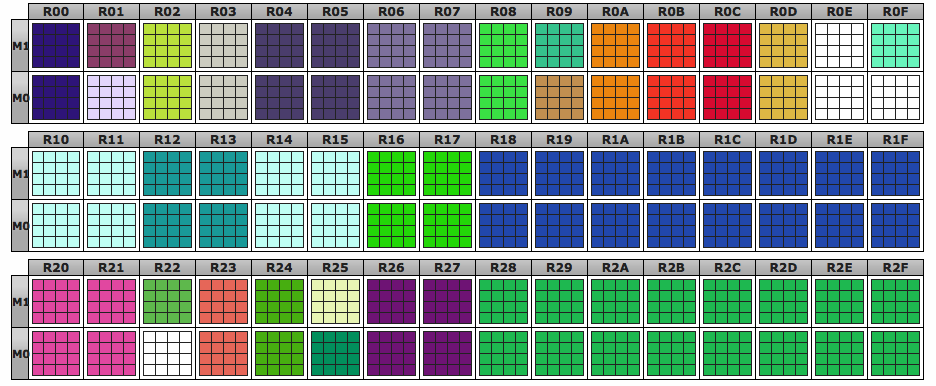
\includegraphics[width=0.38\textwidth]{figs/mira}
   \caption{The activity of Mira, IBM BlueGene/Q system at Argonne National Lab. Many jobs runninng concurrently on the system. Different jobs represented by specific colors. }
   \label{fig: mira activity}
\end{figure}

One of the most prominant problem comes into researcher's attention is the network contention between concurrently running jobs. The network sharing between concurrently running jobs cause communication variability, which reslut in jobs running slower and longer waiting time for results. The delay of currently running jobs will increase the queueing time of the following submitted jobs, thus leads to low system throughput, low utilization and high energy cost. The network sharing can even cause interference between neighbouring jobs, abort the the running job unexpectedly, or even worse, wrong science results. 


This adverse effect of network sharing can be mitigated by providing the job with better node allocation. The batch scheduler is responsible for assigning job with the amount of node it required upon submission. Currently two scheduling strategies are commonly used on torus-connected systems. One is so called partition based systems, where the scheduler assigns each user job a compact and contiguous set of computing nodes. IBM Blue Gene series systems fall into this category. This strategy is in favor of application’s performance by providing it with isolated partition and exclusive network connections, thus reducing network contention caused by concurrently running jobs sharing network bandwidth. However, this strategy can cause internal fragmentation (when more nodes are allocated to a job than it requests) and external fragmentation(when sufficient nodes are available for a request, but they can not be allocated contiguously), therefore leading to poor system performance (e.g., low system utilization and long waiting time for job). The other is non-contiguous allocation system, where free nodes are assigned to user job no matter whether they are contiguous or not. Cray XT/XE series systems fall into this category. Non-contiguous allocation eliminates internal and external fragmentation as seen in partition-based systems, thereby leading to high system utilization. Nevertheless, it introduces other problems such as scattering application processes all over the system and causing both inter-job contention and intra-job contention. The non-contiguous node allocation can make inter-process communication less efficient and cause network contention among concurrently running jobs, thereby resulting in poor job performance especially for those communication-intensive jobs.


Partition-based allocation achieves good job performance by sacrificing system performance (e.g., poor system utiliza- tion), whereas non-contiguous allocation can result in better system performance but could severely degrade performance of user jobs (e.g, prolonged wait-time and run-time). Supercomputers keep growing in size, its network become more sophisticated then ever before and applications also increase its complexity. How to provide application with better allocation that can balance job performance with system performance become a prominant problem need a solution before HPC enters era of exasacle computing. In this work, we propose a guideline for future batch scheduling system, a smart way to make allocation with the awareness of job's communication pattern.

Most existing batch schedulers take so few initiative because it been hold under the obscurantism policy. Whether it use partition-based or non-contigous policy, means it chooses the benefit of either system or job over the other. Some propose compromised policies like buddy system\cite{buddy system paper} still make the allocation for job blindly without knowing job's communication information. 

Although HPC applications complexity continue to grow, people could get more knowledge about the applications communication information with the help from various parallel application profiling tools, such as TAU\cite{tau}, MPIP\cite{mpip} and DUMPI\cite{sst}. Job's communication trace and performance analysis can be get by using such tool at runtime. 

The off-line study of job's communication traces could be helpful to develop better allocation policies for batch scheduler to make on-line scheduling/allocating decisions. This is because the communication pattern of parallel applications on HPC system can be summarized into a couple of categories\cite{hpdc2015-ornl}. The deep understanding of one application can be helpful to all other applications that conforms to the same communication pattern. Job's communication traces study would be extreme helpful to leadership computing facility too. The set of applications running on those leadership computing facilities is usually stable, and the workloads from those HPC systems is usually has great repetitiveness. We analyzed the workload on Mira, an IBM Blue/Gene Q system at Argonne Leadership Computing Facility, found that most jobs require 2k nodes and about 14 particular jobs consist of the majority its workload\ref{fig: repetitiveness of Mira}. In other word, Mira accommodates mostly some particular 14 jobs and most jobs have the same size.


In this work, we present a guideline for future batch scheduler to make allocation with awareness about job's communication pattern. Rather than choose blindly between partition-base or non-contigous allocation, the new allocation mechanism make allocation based on job's communication pattern. With detail analysis about application's communication pattern, we can get a clear view of its communication topology graph, data transfer between processes, and decide which processes are tightly connected to which and conduct intensive communication. The "local community" consists of such tightly coupled processes shuld get compact alloction. Then, the allocation mechanism should make allocations that only needs to guarantee the locality of the subset of the nodes where those "local community" should reside on.

We first pick three signature applications from DOE Design Forward Project\cite{design forward webpage} as examples to conduct deep study about their communication patterns. We identify the "local community" in these applications and assign them allocation accrodingly. The advantage of making allocation is obvious. First, compared with partition-based policy, our communication pattern aware policy is more flexible, it doesn't require the system to provide a big partition that can accomodate the whole application, just small set of compact nodes enough for all the "local community" in the application. On the other hand, our communication pattern aware allocation policy won't destroy the locality of application's communication pattern. On the contrary, it provides small compact node sest for the the "local communities" in the application will preserve the communication locality in the maximum extent.

We use a sophisticated simulation toolkit named CODES, Co-Design of Multi-layer Exascale Storage Architecture, from Argonne National Lab as research vehicle to evaluate the performance of our communication pattern aware allocation policy on torus network. CODES enables the exploration of simulating different HPC networks with high fidelity\cite{Jason-2011}. We extend CODES with a Job Mapping API that support different allocation policies on torus network.

We also conduct a case study with the results we got from communication pattern aware allocation policy evaluation with real trace from production system.\textcolor{red}{Not Sure About this part!!!}

The rest of this paper orgainzed as follows. Section\ref{sec:application study} gives a detailed study of the three applications from DOE Desgin Forward Project. Section\ref{sec:simulation} talks about the simulation platform and Section




\section{Application Study}
\label{sec:application study}

A parallel application usuall conforms to a combination of several basic communication patterns. At its different execution phases, the application's communication behavior may follow different basic patterns repectively. When we look into the data flow during the application execution, most parallel application start with broadcast operation to distribute the data from root process to other processes, followed by a series of computation and communication that comforms to certain pattern, which is usually the dominant part of application's execution. And before the application come to completion, all the working process will return their results to the root dirctly or hierarchically. In this work, we focus on the dominant communication pattern because that's where the application spend most of its running time. We believe making optimized allocation regarding application's dominant communication pattern would greatly benefit both the application and the system. In this section, we analysis two applications whose dominant communication patterns are most prevalent in scientific computation.

There are many profiling tools available to capture the communication behavior from parallel applications, such as Tuning and Analysis Utilities(TAU)\cite{tau}, mpiP\cite{mpip}. They can help analysis parallel application, providing information like the percentage of different MPI operations of the applications, communication topology, the amount data transferred between processes.

In this work, we provide detailed analysis about the communication pattern of two DOE MiniApps. MiniApps are reduced proxy applications that encapsulate the salient performance of larger full size applications\cite{miniapp}. Since we only focus on the dominant communication pattern of parallel applications, these MiniApps are perfect candidates for analysis the application's performance on different allocations or on new network architectures.


\subsection{AMG}
\label{sec:amg}
AMG is the MiniApp of Algebraic Multigrid Solver, which is a parallel algebraic multigrid solver for linear systems arising from problems on unstructured mesh physics packages. It has been derived directly from the BoomerAMG solver that is being developed in the Center for Applied Scientific Computing (CASC) at LLNL\cite{amg}. The dominant communication pattern is this regional communication with decreasing message size for different parts of the multigrid v-cycle.

\begin{figure}[h!] 
  \centering
  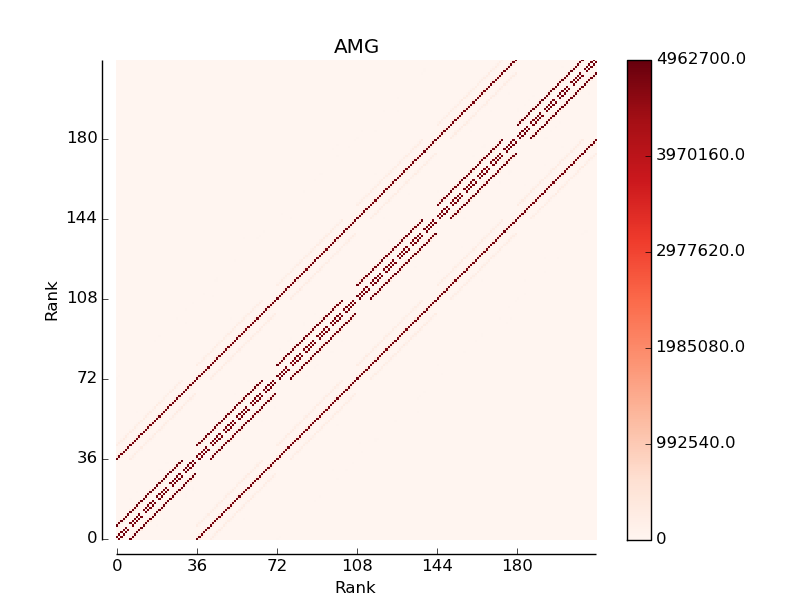
\includegraphics[width=0.38\textwidth]{figs/appstudy/amg/amg_ct}
   \caption{Communication Topology of AMG with 27 MPI Ranks }
   \label{fig: amg communication topology}
\end{figure}

\begin{figure}[h!] 
  \centering
  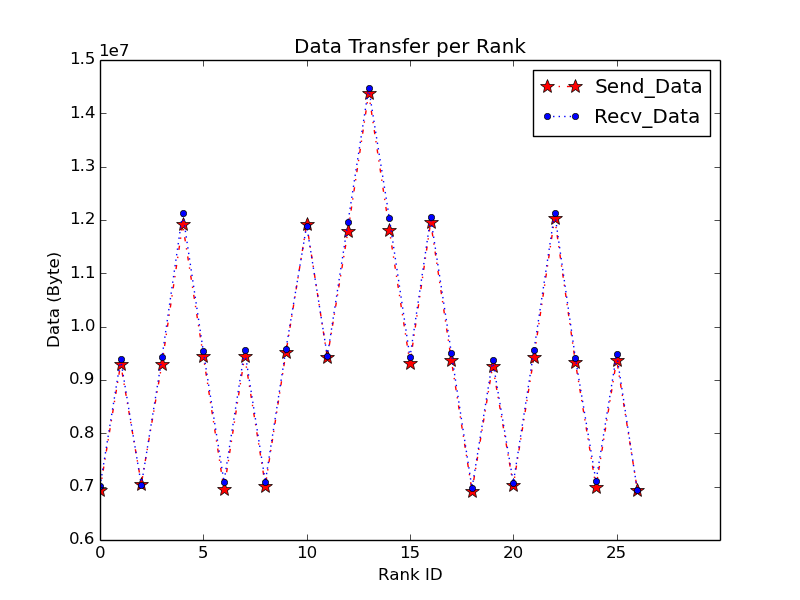
\includegraphics[width=0.38\textwidth]{figs/appstudy/amg/amg_data_transfer}
   \caption{The amount of data each rank transferred in AMG. }
   \label{fig: amg data trans}
\end{figure}

Figure \ref{fig: amg communication topology} shows the communication topology of a small scale AMG with 27 MPI Ranks. Here we prefer to show the communication topology with small scale version of the MiniApp because the dominant communication pattern of the application doesn't change with its scale. We can make the observation from the upper-left of the figure that each rank in AMG has intense communication between 3 other ranks, such as rank 0 between rank 1, 3 and 9, rank 1 between 2, 4 and 10, etc. And this relation is also symmetric along the main diagnal. The dominant communication pattern is quite obvious when we identify this relation between ranks.

Figure \ref{fig: amg data trans} shows the amount of data each rank transferred in AMG. The blue line shows that total data amount transferred from each rank, while the red shows the amount of received data and green shows the amount of send data. The first thing we can spot from the figure is that for each rank, the amount of data sent and received are basically the same, which also well explain the symmetry of the application's dominant communication pattern. And the second thing we can find about AMG is that the data transfer amount also has a symmetric pattern. Rank 0 has the same amout of data transfer as Rank 26, Rank 1 as of Rank 25, etc.


\subsection{Crystal Router}
\label{sec:crystalrouter}

The second MiniApp we have is Crystal Router, which is the extracted communication kernel of the full application Nek5000. Nek5000\cite{crystalrouter} is a spectral element CFD application developed at Argonne National Laboratory. It features spectral element multigrid solvers coupled with a highly scalable, parallel coarse-grid solver that widely used for projects including ocean current modeling, thermal hydraulics of reactor cores, and spatiotemporal chaos. The MiniApp of Nek5000, Crystal Router demonstrates the "many-to-many" communication pattern through scalable multi-stage communication process.

\begin{figure}[h!] 
  \centering
  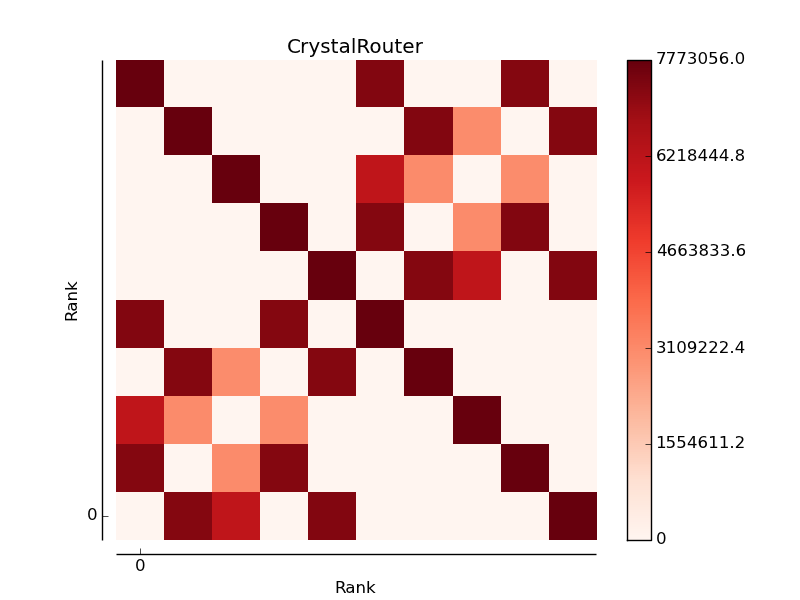
\includegraphics[width=0.38\textwidth]{figs/appstudy/cr/cr10_ct}
   \caption{Communication Topology of Crystal Router with 10 MPI Ranks }
   \label{fig: crystalrouter10 communication topology}
\end{figure}

\begin{figure}[h!] 
  \centering
  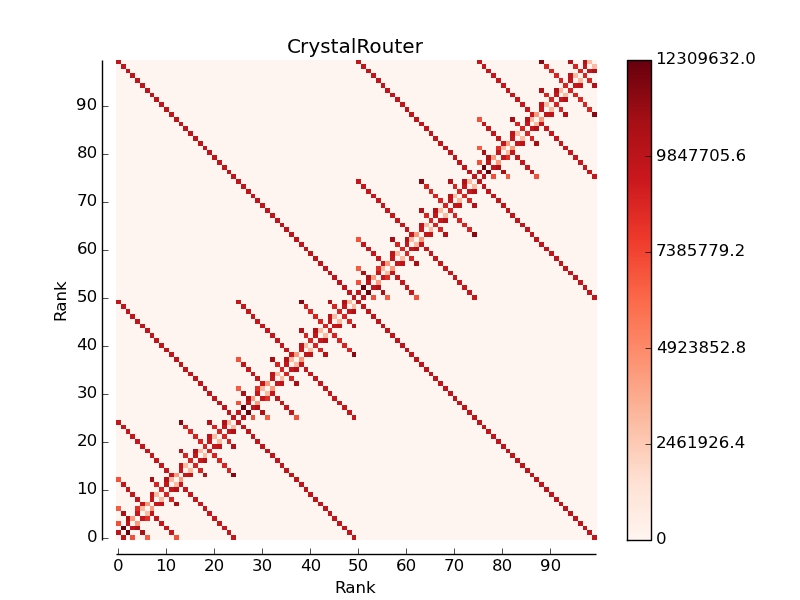
\includegraphics[width=0.38\textwidth]{figs/appstudy/cr/cr100_ct}
   \caption{Communication Topology of Crystal Router with 100 MPI Ranks }
   \label{fig: crystalrouter100 communication topology}
\end{figure}

\begin{figure}[h!] 
  \centering
  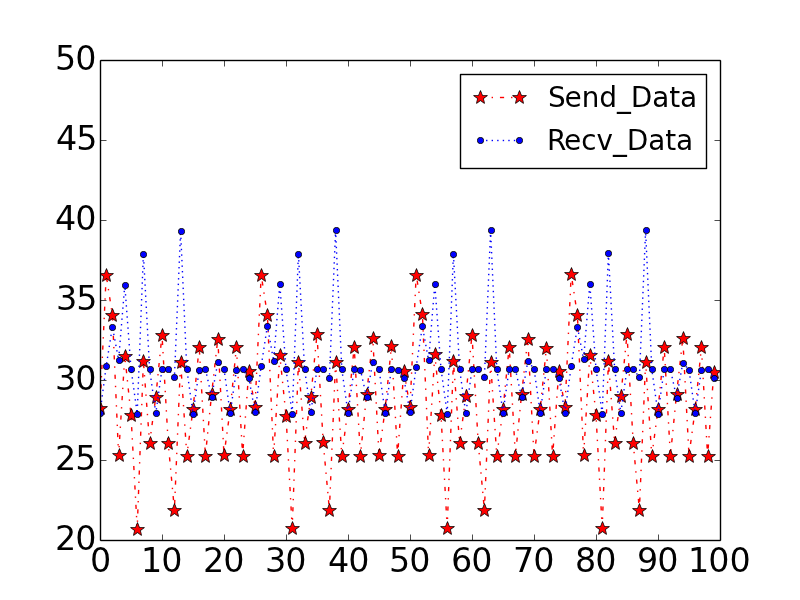
\includegraphics[width=0.38\textwidth]{figs/appstudy/cr/cr_data_transfer}
   \caption{The amount of data each rank transferred in Crystal Router. }
   \label{fig: cr data trans}
\end{figure}

Here, we provide the communication topology graph of Crystal Router with 10-rank and 100-rank respectively. As we can see from figure \ref{fig: crystalrouter10 communication topology}, every 5-rank is a compact community, where data transfer is very intensive. Beside the "5-rank community", there is "pair-wise" global data transfer in Crystal Router. Obviously, there is data transfer alone the diagnal. When the scale of Crystal Router increase to 100, the "5-rank community" is still the dominant pattern in a multi-stage manner. The same pattern can be observed from the global data transfer. Our observation about the dominant communication pattern of Crystal Router is the multi-stage "5-rank community" and "pair-wise" global data transfer happen recursively as the scale of the application increase.

Figure \ref{fig: cr data trans} shows the amount of data each rank transferred in Crystal Router. The locality pattern of "5-rank community" can still be spotted in this figure. The spiky shape occurs in the frequency of every 5 rank. Unlike AMG, the there is variance between the amount of data send and received for each rank. This is due to the specific feature of Crystal Router's communication pattern.


\subsection{MultiGrid}
\label{sec:multigrid}

Differe from AMG, MultiGrid is geometric multigrid v-cycle from production elliptic solver BoxLib, a software framework for massively parallel block-structured adaptive mesh refinement (AMR) codes. MultiGrid conforms to 3D lattice communication pattern with decreasing message size and collectives for different parts of the multigrid v-cycle. It is widely used for structured grid physics packages.

\begin{figure}[h!] 
  \centering
  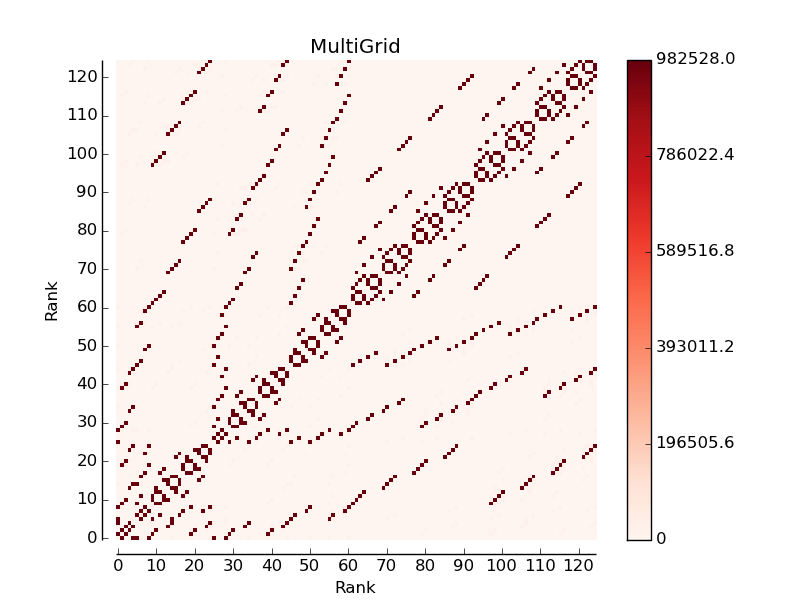
\includegraphics[width=0.38\textwidth]{figs/appstudy/mg/mg125_ct}
   \caption{Communication Topology of MultiGrid with 125 MPI Ranks }
   \label{fig: multigrid125 communication topology}
\end{figure}

\begin{figure}[h!] 
  \centering
  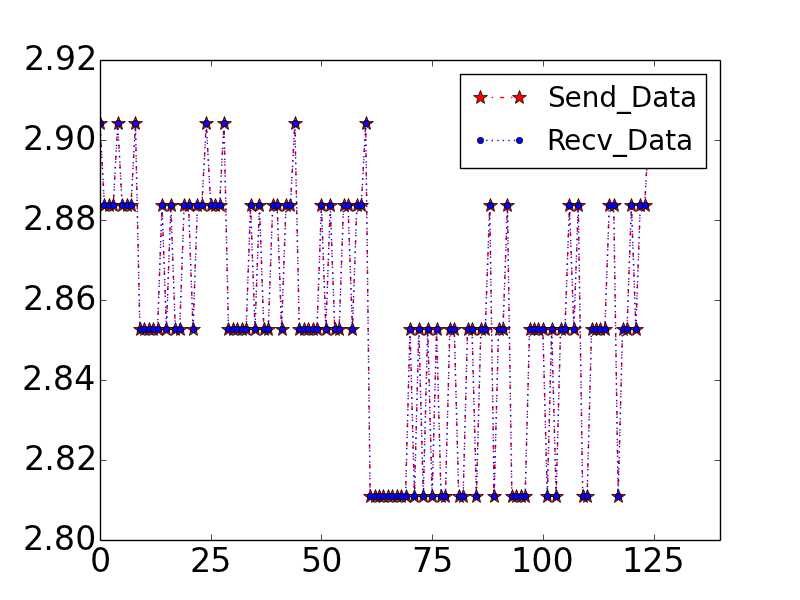
\includegraphics[width=0.38\textwidth]{figs/appstudy/mg/mg_data_transfer}
   \caption{The amount of data each rank transferred in MultiGrid. }
   \label{fig: cr data trans}
\end{figure}


\section{Simulation Platform}
\label{sec:simulation}

A simulation toolkit named CODES (Co-Design of Multi-layer Exascale Storage Architecture) from Argonne National Lab enables the exploration of simulating different HPC networks with high fidelity\cite{Jason-2011}\cite{mubarak-sc2012}. CODES is built on top of Rensselaer Optimistic Simulation System (ROSS) parallel discrete-event simulator, which is capable of processing billions of events per second on leadership-class supercomputers\cite{ross}. CODES support both torus and dragonfly network with high fidelity flit-level simulation. In this work, we only use torus network to show the impact of node allocation to job with different dominant communication patterns. CODES has this network workload component that capable of conducting trace-driven simulation. It can take real MPI application trace generated by SST DUMPI\cite{sst} to drive CODES network models. 


Torus networks have been extensively used in the current generation of supercomputers because of their linear scaling on per-node cost and competitive communication performance. The topology of torus network is k-ary n-cube, with $k^n$ nodes in total arranged in an n-dimensional grid having k nodes in each dimension. Each node has 2$\times$ n direct linked neighbor nodes. 

For a job requires $n$ nodes submitted to non-partition based 3D torus-connected system, it gets an allocation of various possible shapes, which could be 3D balanced-cube, 3D unbalanced-cube, 2D mesh, or even 1D list. Figure \ref{fig: allocation} shows some possible allocations for a 64-node job. 3D balanced-cube allocation (in Figure \ref{fig: allocation} as red) is $\{4,4,4\}$, 3D unbalanced-cube allocation is $\{8,4,2\}$(in Figure \ref{fig: allocation} as green), 2D mesh allocation is $\{8,8,1\}$ (in Figure \ref{fig: allocation} as blue).

\begin{figure}[h!] 
  \centering
  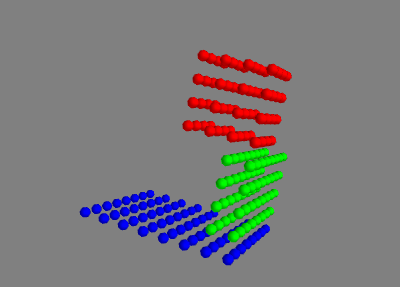
\includegraphics[width=0.48\textwidth]{Pic/allocationshape/allocation}
  \caption{64-node job with different allocation shapes. Red, Green and Blue represents 3D balanced, 3D unbalanced and 2D allocation respectively. }
  \label{fig: allocation}
\end{figure}

We implemented a Job Mapping API for CODES, which can provide flexible job allocation strategies. The new API can help us to explore the impact of different allocation strategies to job with specific communication pattern. We have choosen two publicly available HPC network traces provided by the Design Forward Program\cite{design forward webpage}. The detailed analysis of these two traces are present in Section\ref{sec:amg} and \ref{sec:crystalrouter}.


\subsection{Allocation Simulation}
\label{sec:alloc sim}

In this section, we analysis the impact of different allocation strategies on two real applications, AMG and Grystal Router. The torus network performance is determined by its dimensionality and link bandwidth. We evaluate the data transfer time of AMG and Crystal Router on torus network with different dimensionality and link bandwidth configurations in section \ref{sec: dimensionality study}. Then, we will show applications performance on 3D torus network with different allocation strategies in section \ref{sec: alloc strategy study}.

\subsection{Torus Dimensionality}
\label{sec: dimensionality study}

As the increase of the dimensionality of torus netowrk, so does the number of links connected with each node. The increased aggregated bandwidth of each node will definitely reduce the data transfer time of each rank in the application. Figure xxx shows the performance of the AMG and CrystalRouter on a 2K node torus network model with a 3D torus (16x16x8), a 5D torus (8x4x4x4x4), and a 7D torus (4x4x4x4x2x2x2). The bandwidth between nodes is 2GiB/s in one direction, thus, the aggregated bandwidth is 12GiB/s per node in 3D torus, 20GiB/s per node in 5D torus, and 28GiB/s per node in 7D torus. As we can see from the figure, communication time of both applications decrease as the dimensionality of the network increase. The aggregated bandwidth of each node can accelerate the transfer of data. This can justify the fidelity and consistency of the torus network model.

\begin{figure}[h!] 
  \centering
  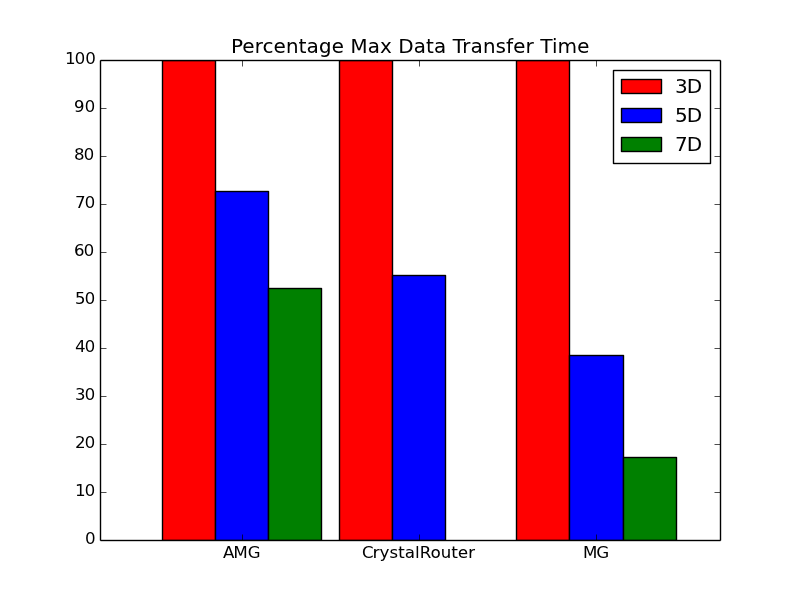
\includegraphics[width=0.38\textwidth]{figs/dimenstudy/maxtime}
   \caption{The Percentage of Maximum Time spent to send data over 3D, 5D and 7D torus networks by AMG1728, CrystalRouter1000, MultiGrid1000.}
   \label{fig: dimenstudy-maxtime}
\end{figure}

\begin{figure}[h!] 
  \centering
  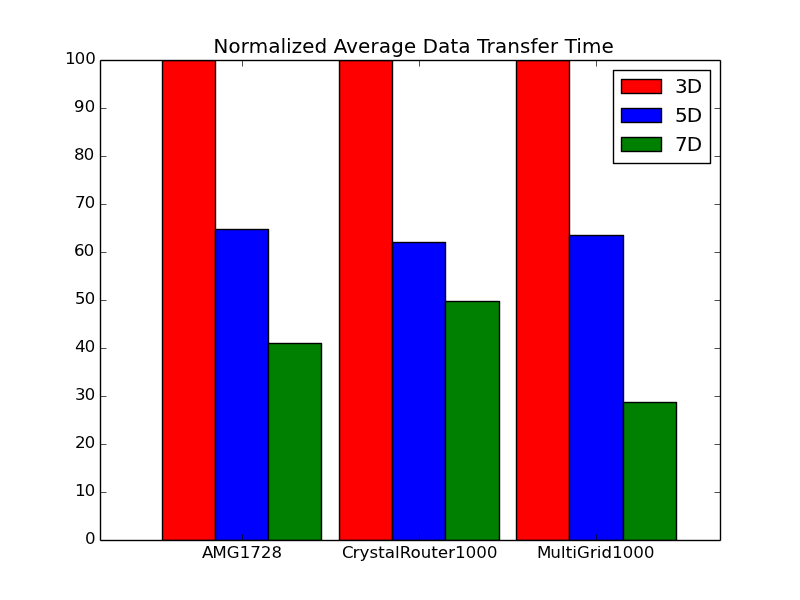
\includegraphics[width=0.38\textwidth]{figs/dimenstudy/avgtime}
   \caption{The Percentage of Average Time spent to send data over 3D, 5D and 7D torus networks by AMG1728, CrystalRouter1000, MultiGrid1000.}
   \label{fig: dimenstudy-avgtime}
\end{figure}

\textcolor{green}{cr1000 on 7D result is missing, will be added soon.}
\textcolor{red}{We can also provide Per-Rank time spent for data transfer. not sure if necessay.}


\section{Communication Pattern Aware Allocation Policy }
In this section, we will explore the performance of three applications on different allocations in a 3D torus network. First, we analysis the impact from different allocation shape, then we will present the results by using our communication aware allocation policy.  

\subsection{Different Allocation Shape}
As we shown in Fig\ref{fig: allocation}, there could be three differet allocation shape on 3D torus network, namely 3D balanced, 3D un-balanced, and 2D. In this section, we will show the performance of three applications on these three different shape allocations.

There are lots of research work try to design fancy allocation algorithms to provide application with most compact allocation, like using space filling curve (SFC) to index high dimentional cube into one dimensional list. Allocation by cutting chunks of nodes from this one dimensional list will guarantee cubical allocation. However, try to provide cubical allocation without considering application's communication pattern could cause backfire.

\textcolor{red}{Detail explanation will be add for Fig\ref{fig: shapestudy-avgtime}-Fig\ref{fig: shapestudy-mg125}.}

\begin{figure}[h!] 
  \centering
  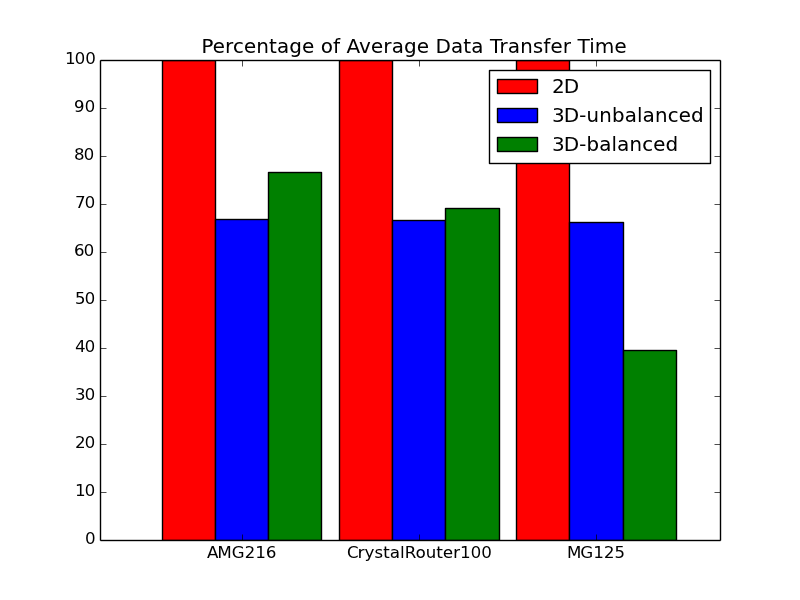
\includegraphics[width=0.38\textwidth]{figs/shapestudy/avgtime}
   \caption{The Percentage of Average Time spent to send data by AMG216, CrystalRouter100, MultiGrid125 with 2D, 3D-unbalanced, 3D-balanced allocation.}
   \label{fig: shapestudy-avgtime}
\end{figure}

\begin{figure}[h!] 
  \centering
  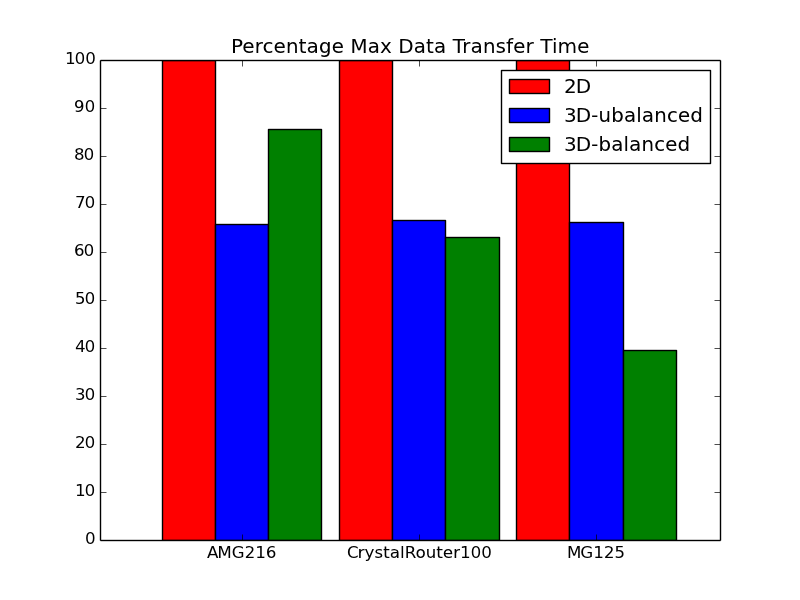
\includegraphics[width=0.38\textwidth]{figs/shapestudy/maxtime}
   \caption{The Percentage of Max Time spent to send data by AMG216, CrystalRouter100, MultiGrid125 with 2D, 3D-unbalanced, 3D-balanced allocation.}
   \label{fig: shapestudy-maxtime}
\end{figure}

\begin{figure}[h!] 
  \centering
  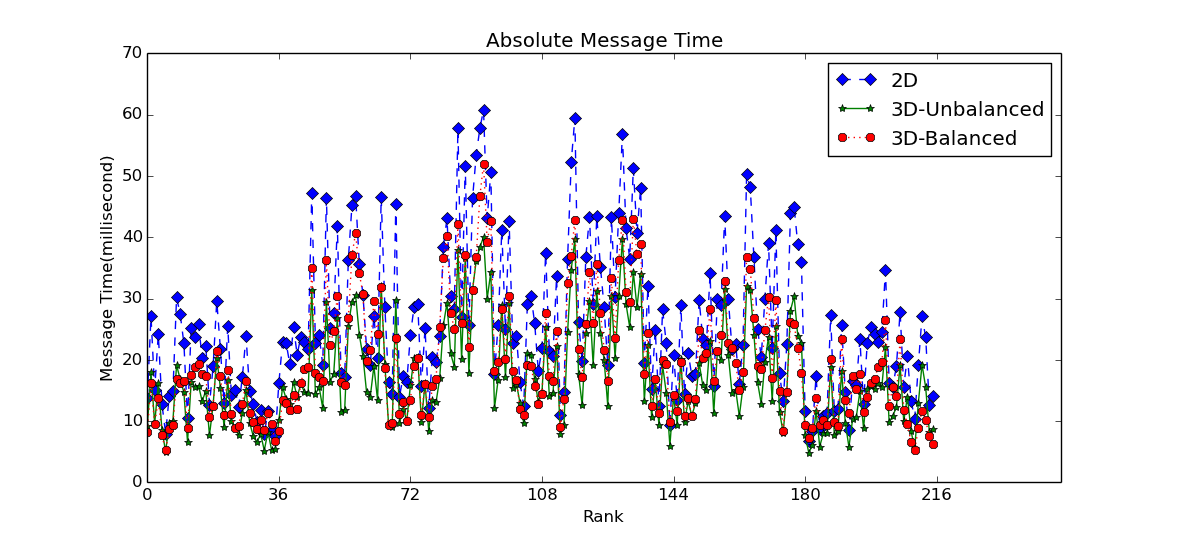
\includegraphics[width=0.38\textwidth]{figs/shapestudy/amg216_rank_msgtime}
   \caption{(AMG216) Time spent by each rank to send data on 2D, 3D-unbalanced, 3D-balanced allocation. }
   \label{fig: shapestudy-amg216}
\end{figure}

\begin{figure}[h!] 
  \centering
  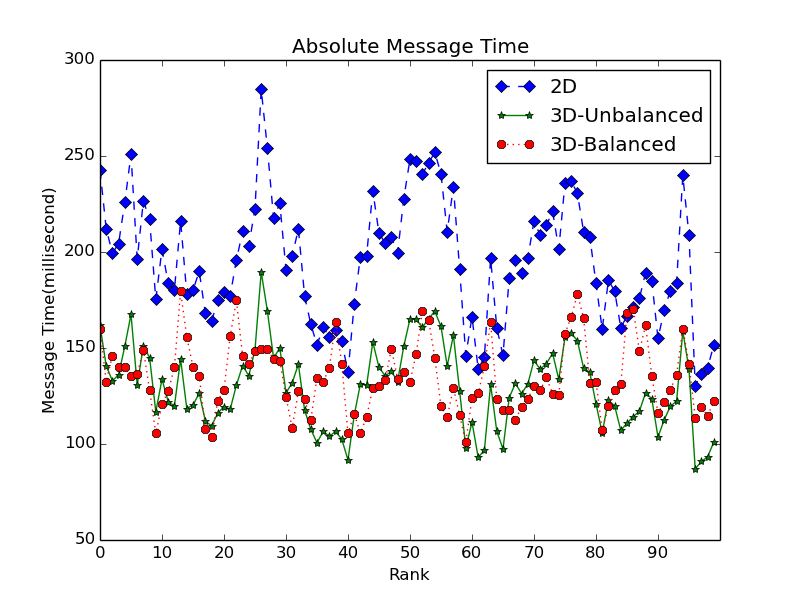
\includegraphics[width=0.38\textwidth]{figs/shapestudy/cr100_rank_msgtime}
   \caption{(CrystalRouter100) Time spent by each rank to send data on on 2D, 3D-unbalanced, 3D-balanced allocation.}
   \label{fig: shapestudy-cr100}
\end{figure}

\begin{figure}[h!] 
  \centering
  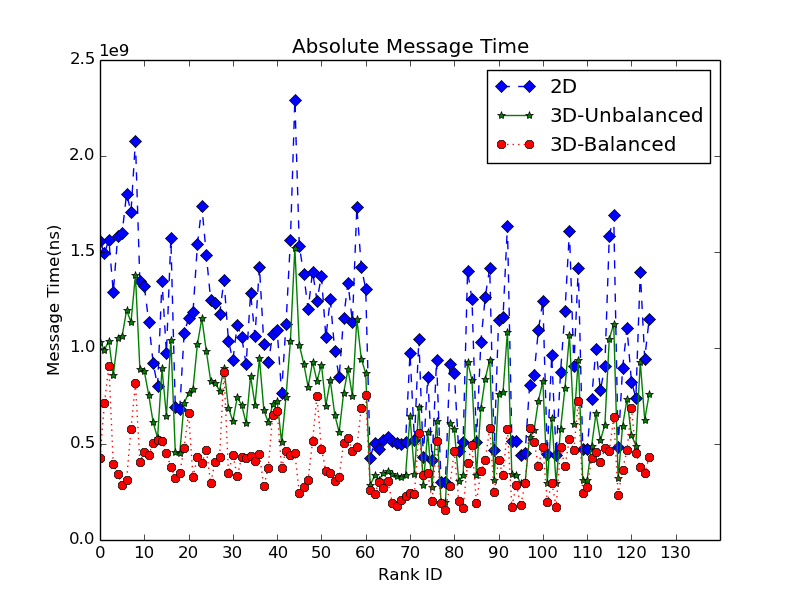
\includegraphics[width=0.38\textwidth]{figs/shapestudy/mg125_rank_msgtime}
   \caption{(MultiGrid125) Time spent by each rank to send data on 2D, 3D-unbalanced, 3D-balanced allocation.}
   \label{fig: shapestudy-mg125}
\end{figure}

\subsection{Allocation Strategies Study}
\label{sec: alloc strategy study}

We proposed two allocation strategies, Compact and Chunk to study the impact of different allocation the application's performance. The Compact allocation always provides application with a cubical allocation on 3D torus, regardless application's communication pattern. This cubical allocation will keep the locality of the application, all the processes reside on it will have the shortest pair-wise distance. 

The Chunk allocation simulation the scenario of non-contiguous allocation strategy employed in production system like Cray XT machines. The traditional non-contiguous allocation simply picks available nodes in spite of their locations and assign them to application. The motivation of non-contiguous allocation act like this is to maximize system utilization, while being blind to application's communication pattern would greatly prolong application's communication time. Although Chunk allocation provides application with non-contigous allocation too, it assign the chunk of nodes in consideration of application's communication pattern. For example, we know the dominant communication pattern of CrystalRouter in section \ref{sec:crystalrouter}, every 5 rank form a community, where intensive communication happens between them. With such knowledge knowledge about application's communication pattern, the Chunk allocation will provide CrystalRouter with allocation that consists of small chunks, the size of which will be at least 5 nodes. 

Figure xxx shows the performance of AMG and CrystalRouter on 3D torus with Compact and Chunk allocation. 






\iffalse

\section{Scheduling Mechanism}
\label{sec:scheduling mechanism}

Figure \ref{fig:overall design} shows the overall design of our new scheduling framework. It takes not only job size, user estimated runtime, but also job's communication pattern (CP) as input parameters. The CP here is provided by user, which indicate the most dominant communication pattern of the user job. The detailed amount of communication data is neither necessary nor possible in this communication pattern. As we show in section \ref{sec:alloc sim} , job with different CP has different preference about network requirement, hence different preference about allocations. For example, job with All-to-All communication pattern requires more network resource, which means a compact or torus allcoation will guarantee a better performance. However, job conforms to Nearest Neighbor communication pattern won't fully utilize the torus network or compact allocation, which means a mesh allocation will serve it equally well.


\begin{figure}[h!]     
\centering  
\includegraphics[width=0.48\textwidth]{Pic/design/overalldesign}  
\caption{Overview of our new scheduling framework. It takes not only job size, user estimated runtime, but also job's communication pattern matrix as input and combines these user provide information with system information to make optimal prioritizing and allocation decisions. It also maintains hashtable, which provides quick reference for making the specific allocation for incoming job with distinct communication pattern. }
\label{fig:overall design}
\end{figure}


Since HPC workload tend to be repetive, our new scheduling framework keep record of historic jobs information to provide quick reference for making the preferable allocation for incoming job with distinct communication pattern. When user submit his job, our new scheduler will first look for job's user name and executable file name in historic record to check whether this job been submitted before. Then the scheduler gets the job's input parameter \{S, CP, ERT\} (job size, Expected RunTime, CommunicationPattern),  and check in the historic data to identify its preferred allocation. As time goes by, our new framework will gradually build up a comprehensive record of all the possible job submission, which is helpful to provide quick reference for the future jobs. Due to the repetitiveness of the workload, the size of this record will grows rapidly at first, then gently grow for a while and come to stagnation, as shown in figure
\ref{fig:table size growth}. 

%\begin{figure}[h!]     
%\centering  
%\includegraphics[width=0.48\textwidth]{Pic/design/tablesize}  
%\caption{The size growth of historic submitted job records.}
%\label{fig:table size growth}
%\end{figure}


We implement a record mechanism as the central component in our framework to keep track of the pattern in workload repetitiveness, hence make predictive optimizations in terms of both job and system performance. Firgure \ref{fig:scheduling mechanism} shows the overview of our design. The scheduler start to build the table since the first submitted job. When user submit a job, the scheduler get job's size and communication pattern, then check the record to find the best allocation for the job. On the other hand, the available resource will be categorized and organized into different types, such as 3D balance, 3D unbalance, 2D balance, 2D unbalance (toruse or mesh). All these available resource will be updated with real-time system feedback information. When a job is finished, the resource it released can be merge into the neighboring one (if the neighbor is also available) to come up with a bigger chunk. So the 2D resource can become into 3D by merging with newly released ones, so does mesh to torus.

%\begin{figure}[h!]     
%\centering  
%\includegraphics[width=0.48\textwidth]{Pic/design/referencetable}  
%\caption{overview of scheduling mechanism}
%\label{fig:scheduling mechanism}
%\end{figure}

With the feedback from system, our scheduling framework will become knowledgeable about the preference of jobs with different communication pattern. The feedback information keep the batch scheduler updated with the latest status of the system such as the number of available nodes, their layout and geometry,  when hotspot or bottleneck come up in network, etc. The scheduler schedule/dispatch the following jobs adaptively based these information.


Our new scheduling framework is designed based on the knowledge about the precognition of workload. The scheduler works periodically and take 3 steps in each scheduling cycle. The scheduling cycle can be predefined by a fixed time interval, or triggered by events like job completion. The 3 steps within each scheduling cycle are

\begin{itemize}

    \item \textbf{Update resource lists from system feedback}. The resource management module take the feedback information form system and refresh the resource lists every time there is a job completes. The resource released by the job can be merged with any other available resource adjacent to it, in order to form up more compact resources. This is similar to Garbage Collection mechanism in memory management. 1D or 2D resource can become 3D resource and unbalance resource become balance resource after being merged with others. The resource list is well organized when the update is finished, thus, better job scheduling 
    
    \item \textbf{Job prioritization and allocation}. With job's information like size, expected runtime, dominant communication pattern provided upon submission and the well organized resource list maintained by resource management module, our scheduler will make decision about timing and location of each job being dispatched to the system. The scheduling policy will be discussed in detail in \ref{sec:scheduling policy}.

    
    \item \textbf{Update reservation}. When a job couldn't get its optimal reousrce allocation and any available suboptimal allocation can not compensate the job's performance lose, the job has an option to make reservation for its optimal resource. Therefore, each time a job got dispatched, the scheduler need to update the reservation, delete those that been satisfied and reserve for the following jobs if necessary.


\end{itemize}



\section{Scheduling Policy}
\label{sec:scheduling policy}

We designed and implemented two scheduling algorithms, Rackless and Cautious, for our new scheduler framework. Both of them take advantage of the scheduler's workload precongnition ability and can deliver comparable performance improvement 
as against the traditional schedulers. The comparision results are presented in \ref{sec:scheduling results}.


Before we introduce our scheduling policy, we will first give explanation about workload and system. Suppose the system has 3D torus network and the available resource is consist of a set of 3D or 2D sub-torus chunks, which can be denoted by $\{v\}$, each $v_i = \{x_i, y_i, z_i\}$. The size of each chunk $v_i$, $S_{v_i} = x_i\cdot y_i\cdot z_i $. 

The job set in the scheduling window is denoted by $\{J\}$, each $J_i$ has size $S_{J_i}$. Due to the repetitiveness of the workload, $S_{J_i} \in \{n_1, n_2, .., n_k\}$, where $k \leq 5$. 
We can make two reasonable assumption about $\{v\}$ and $\{J\}$. 

\begin{equation}
\label{eq:mod0}
\exists S_{v_i} > S_{v_j} \quad then\quad S_{v_i} \bmod S_{v_j} \equiv 0
\end{equation}


\begin{equation}
\label{eq:nofrag}
\min S_{J_i} \leq \min S_{v_i} 
\end{equation}

The reason for both Equation \ref{eq:mod0} and \ref{eq:nofrag} stand is the repetitiveness of workload.


\subsection{Repetitive Job Submission}
\label{sec: repetitive job submission}

The same application could run repetitively on HPC system. This is due to users from some scientific areas have to run the same application multiple times with different configurations. For example, some bioinformatics applications need to conduct the same computation i.e. protein sequence alignment, for a large sets of protein sequences. From system's perspective, all these submissions are the same (same computation instructions and communication phases). Therefore, we can observe the same job multiple times with slightly different input parameter, and all these jobs usually belong to the same user. To substantiate our claim, we analyze the workload trace in 2014 from Mira, an IBM Blue/Gene Q system. As it shown in figure \ref{fig: repetitiveness of Mira},  we list the number of total submissions from five most active users and the percentage of the repetitive ones.


\begin{figure}[h!] 
  \centering
  \includegraphics[width=0.38\textwidth]{Pic/JobInfo/repe-mira-2}
   \caption{ The repetitive job submissions on Mira in 2014. The percentage of repetitive submissions from certain user can be as much as 90\%. }
   \label{fig: repetitiveness of Mira}
\end{figure}



\subsection{Scheduling Policy 1: Reckless}
\label{sec:reckless}

Reckless is designed to be responsive. The overhead for Reckless to make scheduling decision is very low, such that it can be competent when system has high job arrival rate. Reckless first pick a job from the scheduling window and check according the job's size and communication pattern if its optimal resource is availbale. The job get run when enough optimal resource is available. However, if there is no enough optimal resource and only enough sub-optimal availale, Reckless will make reservation if job with ATA communication pattern and run job with non-ATA communication pattern anyway. And if there is no enough resource for any job in the scheduling window, Reckless will hold and skip the current scheduling cycle, wait for more resource got released and make scheduling in the next cycle.

\begin{algorithm}
  \label{alg:scheudling1}
  \caption{Reckless}
  \begin{algorithmic}
    \State \{J\}, Job set in the scheudling window
    \State \{v\}, available system resource sets
    \While{\{J\} is not empty}
        
        \If{optimal $v_i$ is available for $j_i$}
            \State run $j_i$ on $v_i$;
            \State delete $j_i$ from \{J\};
            \State update reservation;
        \EndIf
        
        \If{$\exists \bar{v_i}$ satisfy $j_i$ AND $\bar{v_i}$ is not optimal}
            \If{$j_i$ is ATA dominant}
                \State Wait and Reserve $\hat{v_i}$;
            \EndIf
            \If{$j_i$ is not ATA dominant}
                \State run $j_i$ on $\bar{v_i}$;
                \State delete $j_i$ from \{J\};
                \State update reservation;
            \EndIf
        \EndIf
        
        \If{Available \{$v_i$\} $leq$ $forall$$j_i$ requirement}
            \State hold;
        \EndIf
        
    \EndWhile
  \end{algorithmic}
\end{algorithm}


\subsection{Scheduling Policy 2: Cautious}
\label{sec:cautious}

Our second scheduling algorithm named Cautious. The difference between Reckless and Cautious is that, Cautious always make evaluation before it assign job to sub-optimal resources. The most intuitive evaluation metric is job's turn-around time. As shown in \ref{alg: Evaluate}, it will compare the runtime for job on the sub-optimal resource, and the time for waiting optimal resource plus the runtime for job on optimal resource. The result will decide whether the job will run on the sub-optimal resource promptly or wait and reserve for its optimal resource.

The other evaluation metrics for Cautious to make decision in terms of system is the Lose of Capacity(LOC). As we shown before, the optimal resource always requires embazzle more network resource, which further leads to system fragmentation, and thus low system utilization. The system administrator is free to choose the evaluation metrics here based on the system and workload features.


\begin{algorithm}
  \label{alg:scheudling2}
  \caption{Cautious}
  \begin{algorithmic}
    \State \{J\}, Job set in the scheudling window
    \State \{v\}, available system resource sets
    \While{\{J\} is not empty}
           
        \If{optimal $v_i$ is available for $j_i$}
            \State run $j_i$ on $v_i$;
            \State delete $j_i$ from \{J\};
            \State update reservation;
        \EndIf
        
        \If{$\exists \bar{v_i}$ satisfy $j_i$ AND $\bar{v_i}$ is not optimal}
            \If{Evaluate($j_i$, $\bar{v_i}$)}
                \State run $j_i$ on $\bar{v_i}$;
                \State delete $j_i$ from \{J\};
                \State update reservation;
            \Else
                \State Wait and Reserve $\hat{v_i}$;
                \State Choose from \{J\}-$j_i$ do Backfilling;
            \EndIf
        \EndIf
        
        \If{Available \{$v_i$\} $\leq$ $\forall$$j_i$ requirement}
            \State hold;
        \EndIf
        
    \EndWhile
    
  \end{algorithmic}
\end{algorithm}



\begin{algorithm}
  \label {alg: Evaluate}
  \caption{Evaluate($j_i$, $\bar{v_i}$)}
  \begin{algorithmic}
    \State Get $\bar{t}$, the time for job $j_i$ to complete on suboptimal resource $\bar{v_i}$;
    \State Get $\hat{t}$, the time for job $j_i$ to complete on optimal resource $\hat{v_i}$;
    \State Get $\delta{t}$, the time job $j_i$ wait for optimal resource $\hat{v_i}$;
    \If{$\delta{t} + \hat{t} \leq \bar{t}$}
        \State return False;
    \Else
        \State return True;
    \EndIf
    
  \end{algorithmic}
\end{algorithm}

Both Reckless and Cautious has its pros and cons. Reckless is responsive and efficient, but it make scheduling decision lack of thoughts. The job may suffer a long run time when it assign to sub-optimal resource and can lead to potential system fragmentation. Cautious, on the other hand, spends time for evaluation if there is only sub-optimal resource for the job. 



\section{Evaluation Methodology}
\label{sec: evaluation methodology}

We conduct a series of experiments using the traces described in Section \ref{sec:job traces} to evaluate our design as against two most frequently used scheduling/allocation policies. Both of them use FCFS/EASY backfilling for job prioritizing. When it comes to job allocation, the first use contiguous/compact allocation strategy (\textbf{CC}), which means the nodes within the allocation it assigned to every job are spacially contiguous and compact. The partition-based allocation strategy used in IBM Blue Gene series of machines are of this kind. The second use non-contiguous allocation strategy(\textbf{NC}), which means it provide jobs with allocation without consideration about the adjacency of nodes. The nodes within each allocation could be scattered all over the system. Machines from Cray Inc. use similar allocation strategy like \textbf{NC}. Both the traditional \textbf{NC} and \textbf{CC} are agnostic about workload. In the rest of the paper, we use \emph{Reckless}, \emph{Cautious}, \emph{CC} and \emph{NC} to denote our scheduling policies and the default ones.

\subsection{Evaluation Metrics} 
\label{sec:metrics}
We use three scheduling metrics for the evaluation of our scheduling framework as against the default ones. They have been chosen for the quantified analysis of both system and job's performance.

\begin{itemize}
  
  \item \emph{System Utilization Rate}.  System Utilization Rate can be calculated in the following way. Suppose $T$ is the total elapsed time for $J$ jobs, $t_e$  the completion time for job $i$ and $t_s$ be its the start time, and $n_i$ be the size of job $i$, then system utilization rate is calculated as
  
  \begin{eqnarray}\displaystyle
  \dfrac{\sum_{0\leq i\leq J}{(t_e-t_s) \cdot n_i}}{N \cdot T}
  \end{eqnarray} 
  
  \item \emph{Average Wait Time}. For each job, its wait time refers to the time elapsed between the moment it is submitted and the moment it is dispatched to run. This metric is calculated as the average across all the jobs submitted to the system. The batch scheduler should cut job's wait time down as much as possible.
  
   \begin{eqnarray}\displaystyle
    T_{wait} = t_{start}-t_{arrive}
  \end{eqnarray} 
  
  
	\item \emph{Average Job Response time}. Response time refers to the amount of time it take when each job is submitted until it ends, which equals to its wait time plus its run time.
       
  \begin{eqnarray}\displaystyle
    T_{response} = T_{run}+T_{wait}
  \end{eqnarray}   
	
\end{itemize}

A good batch scheduler should always balance system's performance and user job's performance. On one hand, the batch scheduler should be as responsive as possible, so that user job won't wait too long to get served. On the other hand, the batch scheduler should always guarantee a relative high and stable system uilization so that system resource can be fully utilized.


\subsection{CQSim: Trace-based Scheduling Simulator}
%\textbf{\textcolor{red}{This subsection is Self Plagiarized from Cluster14!!!!}}\\

Simulation is an integral part of our evaluation of various allocation policies
as well as their aggregate effects on system utilization, job's wait time and
response time. We have developed a simulator named CQSim to evaluate our design
at scale. The simulator is written in Python, and is formed by several modules
such as job module, node module, scheduling policy module, etc. Each module is
implemented as a class. The design principles are reusability, extensibility,
and efficiency. The simulator takes job events from the trace, and an event could be
job submission, start, end, and other events. Based on these events, the
simulator emulates job submission, allocation, and execution based on specific
scheduling and allocation policies. CQsim is open source, and is available to the
community \cite{Cqsim}.  \\



\subsection{Job Traces}
\label{sec:job traces}
%\textbf{\textcolor{red}{This subsection is Self Plagiarized from Cluster14!!!!}}\\

In this work, we use two real workload traces collected from production
supercomputers to evaluate our design. The objective of using multiple traces is
to quantify the performance of our design when dealing jobs and systems with
different characteristics. The first trace we used is from a machine named Blue Horizon at
the San Diego Supercomputer Center (denoted as SDSC-BLUE in the paper), which
contains 4,830 jobs. The second trace we used is from a IBM Blue Gene/P system
named Intrepid at Argonne National Laboratory (denoted as ANL-Intrepid in the paper)
\cite{par}. This trace contains 2,612 jobs. Figure \ref{fig:jobsizeintowtraces}
summarizes job size distribution of these traces. ANL-Intrepid is used to
represent capability computing where jobs require a large amount of computing
nodes for solving large-scale problems, whereas SDSC-BLUE is used to represent
capacity computing where the system is utilized to solve a large number of
small-sized problems.

\begin{figure}[h!] 
  \centering
  \includegraphics[width=0.38\textwidth]{Pic/JobInfo/job_dist}
   \caption{Job size distribution of ANL-Intrepid and SDSC-BLUE }
   \label{fig:jobsizeintowtraces}
\end{figure}



\fi



\section{Experiment Results}
\label{sec:scheduling results}
%
%\textcolor{red}{all the figs in this section are obsolete!!!}
%
%\begin{figure}[h!] 
%  \centering
%  \includegraphics[width=0.48\textwidth]{Pic/experiment/summary/utilization}
%  \caption{System Utilization got from CC, NC, Greedy, Cautious respectively}
%  \label{fig: uti}
%\end{figure}
%
%
%\begin{figure}[h!] 
%  \centering
%  \includegraphics[width=0.48\textwidth]{Pic/experiment/summary/awt-vs-cc}
%  \caption{Jobs' average wait time reduction got by comparing CC as against our design.}
%  \label{fig: uti}
%\end{figure}
%
%
%\begin{figure}[h!] 
%  \centering
%  \includegraphics[width=0.48\textwidth]{Pic/experiment/summary/art-vs-cc}
%  \caption{Jobs' average response time reduction got by comparing CC as against our design.}
%  \label{fig: uti}
%\end{figure}
%
%\begin{figure}[h!] 
%  \centering
%  \includegraphics[width=0.48\textwidth]{Pic/experiment/summary/awt-vs-nc}
%  \caption{Jobs' average wait time reduction got by comparing NC as against our design.}
%  \label{fig: uti}
%\end{figure}
%
%
%\begin{figure}[h!] 
%  \centering
%  \includegraphics[width=0.48\textwidth]{Pic/experiment/summary/art-vs-nc}
%  \caption{Jobs' average response time reduction got by comparing NC as against our design.}
%  \label{fig: uti}
%\end{figure}



\section{Related Work}
\label{sec:related_work}
Batch scheduling on HPC system has been a hot topic getting constant discussion since the 1990's.
Feitelson et al proposed the most widely used job scheduling policy which is First Come, First Serve (FCFS) combined with 
EASY backfilling\cite{feit}. FCFS/EASY backfilling policy greatly improves HPC system's utilization and cuts the wait time 
of first job in the waiting queue. Since then, many studies seek to refine this classic scheduling paradigm. Tang et al. 
tried to improve the accuracy of user's estimated job runtime and walltime so as to enhance the efficiency of backfilling and  minimize the system fragmentation\cite{wei-ipdps2010} \cite{wei-jpdc2013} \cite{wei-ipdps2011}. % And there are some other variation of FCFS/EASY backfilling proposed to optimize system performance in terms of power consumption and energy cost \cite{zhou}\cite{yang-sc13}.


Only with the information about job size and estimated run time seems to be insufficient for batch scheduler do make the 
optimal scheduling/allocaiton decision. Some work proposed that the batch scheduler should be aware of some information 
about system network information in order to fully utilize system resources.Leung et al. presented allocation strategies 
based on space filling curves and one dimensional packing \cite{leung}. The problem with using space filling curve is that  
it can only be applied to system with the scale of $2^n$ nodes in each dimension, which is a ideal case that not existing 
in morden HPC systems. Albing et al. conducted study about the allocation strategies that the Cray
Application Level Placement Scheduler (ALPS) used \cite{carl-cug}. The job allocation in Cray Linux Environment (CLE) 
operating system is managed by ALPS, which simply works off an ordered node list, however that is ordered. 

Based on their 
work, Yang et al. presented a window-based locality-aware job scheduling design for torus-connected system
\cite{yang-cluster14}. In this new scheduling framework, several jobs are taken into  consideration at the same time for job 
prioritizing and resource allocation. A list of slots is maintained to preserve node contiguity information for
resource allocation. Each job been assigned into one of these slot so that the locality can be mostly preserved.

Rosenthal et al. found there is limited benefit for many applications by
increasing network bandwidth \cite{rosenthal}. They employed a subset of the
CORAL mini-applications that represent U.S. Department of Energy workload and
leverage multirail networkings to evaluate the improvement of these applications
caused by increased network bandwidth. The applications that send mostly small
messages or larger messages asynchronously are not bandwidth bounded, hence,
benefit only slightly or not at all from increased bandwidth.

   

Hoefler et al. propose to use performance modeling techniques to analysis 
factors that impact the performance of parallel scientific applications 
\cite{hoefler-modeling}. However, as the scale of HPC continue grows, the 
interference of concurrently running jobs is getting worse, which is hard to be 
quantified by performance profiling tools.


Bogdan et al provide a set of guidelines how to configure a network with 
Dragonfly topology for workload with Nearest Neighbor communication 
pattern\cite{Bogdan-hpdc14}. They first derived a theoretical model of Nearest 
Neighbor communication performance on Dragonfly network that can predict network 
bottleneck. Then, they use simulation to validate the correctness of their 
theoretical model.

Dong et al describe IBM Blue Gene/Q's 5D torus interconnect
network\cite{Dong-SC11}. They developed simple benchmarks that conforms to four
different communication patterns, namely ping-pong, nearest neighbor, broadcast
and allredcue, to demonstrate the effectiveness of this highly parallel 5D torus
network.



\section{Conclusions}
\label{sec:conclusion}


\section*{Acknowledgment}
\label{sec: ack}
%We appreciate the valuable comments and suggestions from the anonymous reviewers. 
The work at Illinois Institute of Technology is supported in part by
US National Science Foundation grant CNS-1320125. The work at Argonne is
supported in part by the U.S. Department of Energy (DOE), Office of Science,
under Contract DE-AC02-06CH11357.



\begin{thebibliography}{10}
 %=====start of scheduling papers===== 
\bibitem{feit}
D.~Feitelson and A.~Weil.
\newblock Utilization and predictability in scheduling the {IBM} {SP2} with
  backfilling.
\newblock In {\em International Parallel and Distributed Processing Symposium}, 1998.

\bibitem{wei-ipdps2010}
W.~Tang, N.~Desai, D.~Buettner, and Z.~Lan.
\newblock Analyzing and adjusting user runtime estimates to improve job
  scheduling on the {Blue} {Gene/P}.
\newblock In {\em 2010 IEEE International Symposium on Parallel Distributed
  Processing}, 2010.

\bibitem{wei-ipdps2011}
W.~Tang, Z.~Lan, N.~Desai, D.~Buettner, and Y.~Yu.
\newblock Reducing fragmentation on torus-connected supercomputers.
\newblock In {\em 2011 IEEE International Symposium on Parallel Distributed
  Processing Symposium}, 2011.

\bibitem{wei-jpdc2013}
W.~Tang, N.~Desai, D.~Buettner, and Z.~Lan. 
\newblock Job Scheduling With Adjusted Runtime Estimates on Production Supercomputers.
\newblock Journal of Parallel and Distributed Computing (JPDC), 73(7):926-938, 2013.

\bibitem{zhou}
Z.~Zhou, Z.~Lan, W.~Tang, and N.~Desai.
\newblock Reducing energy costs for {IBM Blue} {Gene/P} via {Power-Aware} job
  scheduling.
\newblock In {\em 17th Workshop on Job Scheduling Strategies for Parallel
  Processing}, 2013.

\bibitem{yang-sc13}
X. ~Yang, Z.~Zhou, S.~Wallace Z.~Lan, W.~Tang, S. ~Coghlan and Mike. ~Papka.
\newblock Integrating Dynamic Pricing of Electricity into Energy Aware Scheduling for HPC Systems. 
\newblock In {Proceedings of the International Conference on High Performance Computing, Networking, Storage and Analysis(SC), 2013 International Conference for}
\newblock SC '13,
\newblock 2013,
\newblock Salt Lake City, Utah

\bibitem{Cqsim}
{\textcolor{red} {Cqsim: An event-driven simulator}}.
\newblock http://bluesky.cs.iit.edu/cqsim


%=====start of allocation aware papers===== 
\bibitem{leung}
Leung, V.J.; Arkin, E.M.; Bender, M.A.; Bunde, D.; Johnston, J.; 
Alok Lal; Mitchell, J.S.B.; Phillips, C.; Seiden, S.S., 
\newblock Processor allocation on Cplant: achieving general processor locality using one-dimensional allocation strategies
\newblock In {Proceedings of 2002 IEEE International Conference on Cluster Computing, 2002}.  pages 296--304, 2002

\bibitem{carl-cug}
Carl Albing and Mark Baker
\newblock ALPS,Topology, and Performance: A Comparison of Linear Orderings for 
Application Placement in a 3D torus.
\newblock Presented at the CUG 2010, Edinburgh, Scotland, UK, 2010.

\bibitem{yang-cluster14}
Xu Yang and Zhou Zhou and Wei Tang and Xingwu Zheng and Jia Wang and Zhiling Lan.
\newblock Cluster Computing (CLUSTER), 2014 IEEE International Conference on,
\newblock Balancing job performance with system performance via locality-aware scheduling on torus-connected systems
\newblock Sept, 2014,
\newblock pp.140-148

%+++++++++++++++++++++++
\bibitem{mpip}
\newblock mpiP: Lightweight, Scalable MPI Profiling.
\newblock http://mpip.sourceforge.net, 
\newblock 2013.

\bibitem{tau}
S. Shende and A. Malony. 
\newblock The TAU parallel performance system. 
\newblock International Journal of High Performance Computing Applications, 20(2):287–311, 2006.

\bibitem{scala}
X. Wu, F. Mueller, S. Pakin, 
\newblock "Automatic Generation of Executable Communication Specifications from Parallel Applications", 
\newblock In {Proceedings of the International Conference on High Performance Computing, Networking, Storage and Analysis(SC), 2011 International Conference for}
\newblock SC '11,
\newblock 2011,pages 12-21.

\bibitem{design forward webpage}
Department of Energy, “Characterization of the DOE Mini-apps.” [Online].
\newblock Available: http://portal.nersc.gov/project/CAL/trace.htm
\newblock (Accessed on: Sept 16th. 2015)

\bibitem{miniapp}
Bronson Messer
\newblock "Using a Developing MiniApp to Compare Platform Characteristics on Cray Systems"
\newblock In Proceedings of Cray User Group 2012

\bibitem{amg}
V. E. Henson and U. M. Yang, 
\newblock "BoomerAMG: A Parallel Algebraic Multigrid Solver and Preconditioner",
\newblock Appl. Num. Math. 41 (2002), pp. 155-177. UCRL-JC-141495.

\bibitem{crystalrouter}
P. Fischer, J. Lottes, D. Pointer, and A. Siegel, 
\newblock “Petascale algorithms for reactor hydrodynamics,”
\newblock Journal of Physics: Conference Series, vol. 125, no. 1, p. 012076, 2008.

%+++++++++++++++++

%=====start of network papers===== 
\bibitem{rosenthal}
E. Rosenthal and E.A. Leon
\newblock Characterizing Application Sensitivity to Network Performance.
\newblock  In {Proceedings of SC14: International
Conference for High Performance Computing, Networking, Storage and Analysis},
2014

\bibitem{hoefler-modeling}
T. Hoefler and W. Gropp and M. Snir and W. Kramer
\newblock Performance Modeling for Systematic Performance Tuning,
\newblock 2011
\newblock Nov.
\newblock In {Proceedings of International Conference for High Performance Computing, Networking, Storage and Analysis (SC'11), SotP Session,
}

\bibitem{roth}
P. Roth and J. Meredith and J. Vetter,
\newblock "Automated Characterization of Parallel Application Communication Patterns",
In Proceedings of the 25rd International Symposium on High-performance Parallel and Distributed Computing
\newblock HPDC '15,
\newblock 2015,


%=====end of application/mapping papers===== 
\bibitem{Pjesivac}
Pje\v{s}ivac-Grbovi\'{c}, Jelena and Angskun, Thara and Bosilca, George and Fagg, Graham E. and Gabriel, Edgar and Dongarra, Jack J.
\newblock Performance Analysis of MPI Collective Operations,
\newblock Cluster Computing,
\newblock June 2007,
\newblock volume 10,
\newblock numpages 17,
 

\bibitem{thakur}
Thakur, Rajeev and Gropp, William D.
\newblock Improving the performance of collective operations in MPICH,
\newblock Recent Advances in Parallel Virtual Machine and Message Passing Interface,
\newblock year 2003,
\newblock Springer

\bibitem{abhinav-ipdps15}
Abhinav Bhatele, Andrew R. Titus, Jayaraman J. Thiagarajan, Nikhil Jain, Todd Gamblin,
Peer-Timo Bremer, Martin Schulz† and Laxmikant V. Kale,
\newblock "Identifying the Culprits behind Network Congestion",
\newblock In {\em 2015 IEEE International Symposium on Parallel Distributed Processing Symposium}, 2015.

\bibitem{langer}
S. Langer, A. Bhatele, and C. H. Still,
\newblock “pF3D simulations of laser-plasma interactions in National Ignition Facility experiments,” 
\newblock Computing in Science and Engineering, vol. 99, Aug. 2014, lLNL- JRNL-648736. 
\newblock [Online]. Available: http://doi.ieeecomputersociety.org/ 10.1109/MCSE.2014.79

%\bibitem{abhatele-ipdps08}
%A. Bhatele, L.V.  Kale
%\newblock Application-specific topology-aware mapping for three dimensional topologies.
%\newblock In {\em Proceedings of Workshop on Large-Scale Parallel Processing (held as part of IPDPS' 08)} 2008
%
%\bibitem{abhinav-sc13} 
%Bhatele, Abhinav and Mohror, Kathryn and Langer, Steven
%H. and Isaacs, Katherine E. 
%\newblock There Goes the Neighborhood: Performance Degradation Due to Nearby Jobs 
%\newblock In {Proceedings of SC13: International
%Conference for High Performance Computing, Networking, Storage and Analysis},
%2013

\bibitem{hpdc14}
Prisacari, Bogdan and Rodriguez, German and Heidelberger, Philip and Chen, Dong and Minkenberg, Cyriel and Hoefler, Torsten
\newblock Efficient Task Placement and Routing of Nearest Neighbor Exchanges in Dragonfly Networks
\newblock In Proceedings of the 23rd International Symposium on High-performance Parallel and Distributed Computing
\newblock HPDC '14,
\newblock 2014,
\newblock Vancouver, BC, Canada

\bibitem{jingjin}
Wu, Jingjin and Lan, Zhiling and Xiong, Xuanxing and Gnedin, Nickolay Y. and Kravtsov, Andrey V.
\newblock Hierarchical Task Mapping of Cell-based AMR Cosmology Simulations
\newblock Proceedings of the International Conference on High Performance Computing, Networking, Storage and Analysis
\newblock SC '12,
\newblock 2012,
\newblock Salt Lake City, Utah

\bibitem{zhou-ipdps}
Z. Zhou, X. Yang, Z. Lan, P. Rich, W. Tang, V. Morozov, and N. Desai.
\newblock Improving Batch Scheduling on Blue Gene/Q by Relaxing 5D Torus Network Allocation Constraints,
\newblock Proceedings of 29th IEEE International Parallel \& Distributed Processing 
Symposium,
\newblock IPDPS'15, 2015.
\newblock Hyderabad, INDIA

\bibitem{Bogdan-hpdc14}
Prisacari, Bogdan and Rodriguez, German and Heidelberger, Philip and Chen, Dong and Minkenberg, Cyriel and Hoefler, Torsten
\newblock Efficient Task Placement and Routing of Nearest Neighbor Exchanges in Dragonfly Networks,
\newblock Proceedings of the 23rd International Symposium on High-performance Parallel and Distributed Computing,
\newblock HPDC '14,
\newblock 2014,
\newblock  Vancouver, BC, Canada,


\bibitem{hpdc2015-ornl}
Philip. C.R, Jeremy S. M, etc
\newblock "Automated Characterization of Parallel Application Communication Patterns"
\newblock HPDC'15

\bibitem{Dong-SC11}
Dong Chen; Eisley, N.A.; Heidelberger, P.; Senger, R.M.; Sugawara, Y.; Kumar,
S.; Salapura, V.; Satterfield, D.L.; Steinmacher-Burow, B.; Parker, J.J., 
\newblock "The IBM Blue Gene/Q interconnection network and message unit," 
\newblock High Performance Computing, Networking, Storage and Analysis (SC), 2011 International 
Conference,
\newblock pp.1,10, 
\newblock 12-18 Nov. 2011

\bibitem{Jason-2011}
Jason Cope, Ning Liu, Sam Lang, Phil Carns, Chris Carothers, Robert Ross.
\newblock Proceedings of the Workshop on Emerging Supercomputing Technologies 2011,
\newblock 2011


%===simulation papers =====

\bibitem{ross}
P. D. Barnes, C. D. Carothers, D. R. Jefferson, and J. M. LaPre, 
\newblock “Warp speed: executing time warp on 1,966,080 cores,”
\newblock in Proc. of the 2013 ACM SIGSIM Conf. on Principles of Advanced Discrete Simulation (PADS),
\newblock May 2013, pp. 327–336.

\bibitem{mubarak-sc2012}
Mubarak, M.; Carothers, C.D.; Ross, R.; Carns, P.,
\newblock "Modeling a Million-Node Dragonfly Network Using Massively Parallel Discrete-Event Simulation," 
\newblock High Performance Computing, Networking, Storage and Analysis (SCC), 
\newblock 2012 SC Companion: 
\newblock pp.366,376, 10-16 Nov. 2012

\bibitem{sst}
Sandia National Labs, “SST DUMPI trace library.” [Online].
\newblock Available: http://sst.sandia.gov/using dumpi.html 
\newblock (Accessed on: Sept 3rd, 2015)


\end{thebibliography}

\end{document}


